\chapter{Proposed Method: \fcsg}\label{ch:method}

This chapter describes the synthetic degradation used for training and
evaluation, and then the network itself, one module at a time. The notation
follows the implementation in \texttt{models/fcsg.py} and
\texttt{models/blocks.py}.

\section{Degradation Model}\label{sec:degradation}

Archival photographs are degraded in a rough physical order: the lens softens
the image, scanning or resizing loses resolution, the sensor or film adds
noise, and lossy storage compresses whatever is left. Our synthetic pipeline
applies the four operations in that order (Table~\ref{tab:degradation}).
\begin{table}[htbp]
	\centering
	\caption{Composite degradation pipeline. Parameters are sampled independently for every image.}
	\label{tab:degradation}
	\begin{tabular}{@{}lll@{}}
		\toprule
		Stage & Parameter & Distribution \\
		\midrule
		Gaussian blur        & $\sigma_\text{blur}$ & $\mathcal{U}(0.5,\, 2.0)$ pixels \\
		Down/up resampling   & scale $s$            & $\mathcal{U}(1.0,\, 2.0)$, bicubic both ways \\
		Additive noise       & $\sigma_n$           & $\mathcal{U}(5,\, 50)/255$, clipped to $[0,1]$ \\
		JPEG compression     & quality $q$          & integer, uniform on $\{30,\dots,95\}$, 4:4:4 \\
		\bottomrule
	\end{tabular}
\end{table}

Blur uses Pillow's Gaussian filter. Resampling shrinks the image by $s$ with
bicubic interpolation and enlarges it back to the original size, so input and
output always have the same dimensions. Noise is additive white Gaussian noise
in 8-bit units, clipped to the valid range. JPEG encoding uses Pillow with
chroma subsampling disabled. The image is quantised to 8 bits before the
Pillow blur and before JPEG encoding, as a real file would be.

Each sample carries its four sampled parameters alongside the degraded and
clean images. The network never sees them. They are recorded so that, after
training, we can ask whether the router responds to the degradation
(Chapter~\ref{ch:routing}). With noise between 5 and 50 grey levels and JPEG
quality as low as 30, the mean input PSNR on our validation set is
20.99\dB{}.

\section{Architecture Overview}\label{sec:arch}

Figure~\ref{fig:architecture} shows the data flow. The degraded image $x$ is
split into a low, a mid and a high frequency band, each of which is an
ordinary RGB image. Three shared experts with $7\times7$, $5\times5$ and
$3\times3$ kernels process every band. A spatial gate assigns, at each pixel
and for each band, a weight to every expert, keeping only the two largest.
The weighted expert outputs form one restored image per band:
\begin{equation}
	y_b(u,v) = \sum_{e\in\{7,5,3\}} w_{b,e}(u,v)\; E_e(x_b)(u,v),
	\qquad b\in\{L,M,H\}.
	\label{eq:mix}
\end{equation}
The three band outputs are concatenated into nine channels, reweighted by a
squeeze-and-excitation block, projected back to RGB and refined. The network
predicts a residual that is added to its input:
\begin{equation}
	\hat{f} = x + \mathrm{Refine}\big(\mathrm{SEFusion}([\,y_L, y_M, y_H\,])\big).
	\label{eq:out}
\end{equation}

\begin{figure}[htbp]
	\centering
	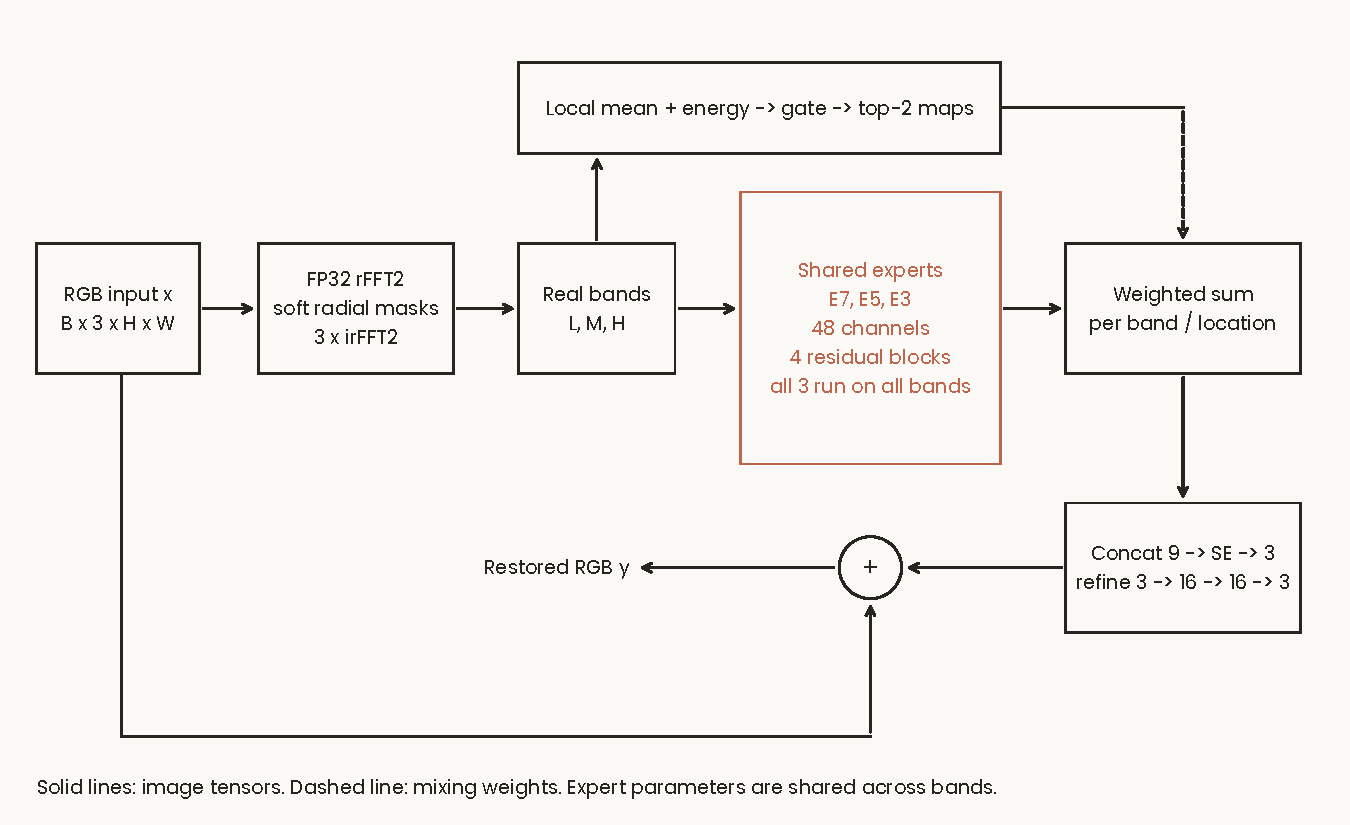
\includegraphics[width=\linewidth]{architecture.pdf}
	\caption{\fcsg{} data flow. Expert parameters are shared across the three
	bands; the band dimension is folded into the batch dimension before each
	expert call.}
	\label{fig:architecture}
\end{figure}

\section{Frequency Decomposition}\label{sec:freqdecomp}

The decomposition is done in the Fourier domain with fixed masks, but the
result of each mask is returned to the spatial domain immediately. We made
this choice early and deliberately. An earlier version of the proposal fed
masked complex spectra straight into the convolutional experts. That has two
problems. A convolution over a spectrum has no clean meaning, since
multiplication in one domain corresponds to convolution in the other, so the
argument that large kernels suit smooth structure no longer applies. And
complex inputs either become two real channels, where phase is discontinuous
and training becomes unstable, or require complex tensor support that many
PyTorch operations lack. Masking in frequency and filtering in space keeps
the decomposition exact and lets every expert be a plain real-valued CNN.

Let $X = \mathcal{F}(x)$ be the two-dimensional real FFT of the image with
orthonormal scaling, and let $r = \sqrt{f_x^2 + f_y^2}$ be the radial
frequency in cycles per pixel. Frequencies are built with \texttt{fftfreq}
and \texttt{rfftfreq} in the unshifted order the FFT uses. Each axis reaches
the Nyquist limit at $0.5$ cycles per pixel. A soft low-pass mask with cutoff
$c$ and transition width $\Delta = 0.05$ is a raised cosine:
\begin{equation}
	t_c(r) = \mathrm{clip}\!\left(\frac{r-c}{\Delta} + \tfrac12,\ 0,\ 1\right),
	\qquad
	\mathrm{LP}_c(r) = \tfrac12\big(1 + \cos(\pi\, t_c(r))\big).
	\label{eq:lowpass}
\end{equation}
With cutoffs $r_1 = 0.10$ and $r_2 = 0.25$, the three band masks are
\begin{equation}
	M_L = \mathrm{LP}_{r_1}, \qquad
	M_M = \mathrm{LP}_{r_2} - \mathrm{LP}_{r_1}, \qquad
	M_H = 1 - \mathrm{LP}_{r_2},
	\label{eq:masks}
\end{equation}
and each band image is $x_b = \mathcal{F}^{-1}(M_b \cdot X)$.

Three properties matter. First, the masks sum to one at every frequency, and
the FFT is linear, so $x_L + x_M + x_H = x$ exactly; no information is lost
or invented by the split. We measured a maximum reconstruction error of
$6.0\times10^{-7}$ in single precision. Second, the cutoffs are defined in
cycles per pixel rather than in FFT bin indices. A bin index means a
different physical frequency at $128\times128$ than at full resolution, so
bin-based cutoffs would shift between training crops and test images. With
normalised radii the same sinusoid falls in the same band at both sizes,
which we verified at 128 and 256 pixels. Third, the transitions are smooth.
A hard step in frequency produces ringing in space, and the network would
spend capacity undoing artefacts of its own preprocessing.

The FFT runs in single precision even during mixed-precision training,
because half-precision CUDA FFTs only support power-of-two sizes.
Figure~\ref{fig:masks} plots the three masks.

\begin{figure}[htbp]
	\centering
	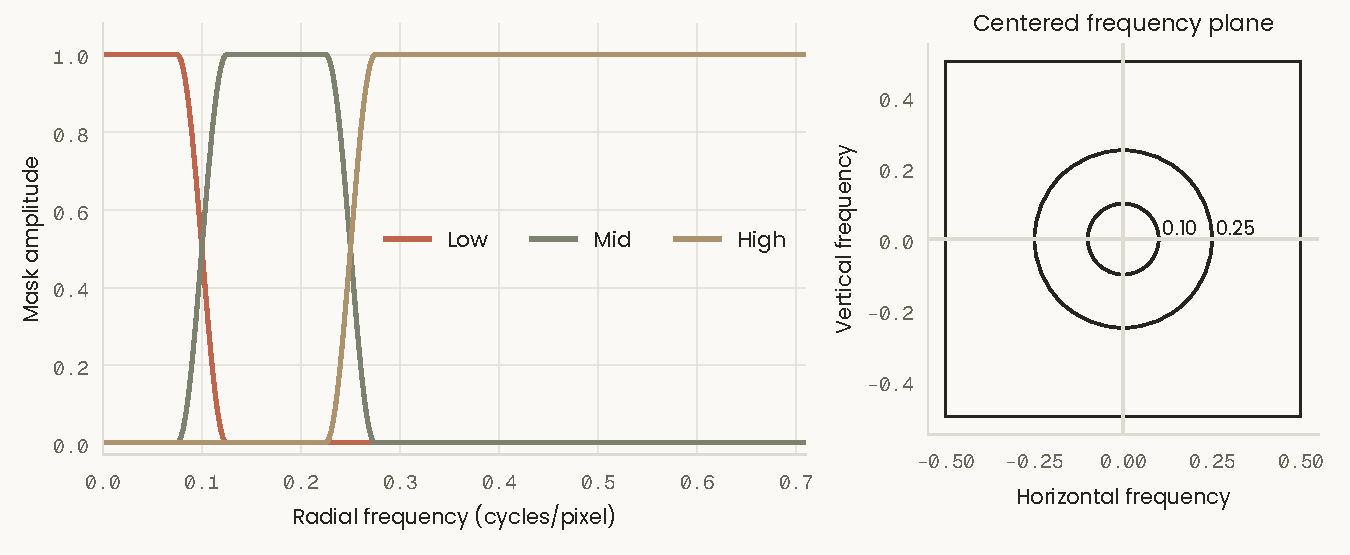
\includegraphics[width=0.9\linewidth]{frequency_masks.pdf}
	\caption{Raised-cosine band masks with cutoffs 0.10 and 0.25 cycles per
	pixel and transition width 0.05. Right: the masks on a centred frequency
	plane (the computation itself uses unshifted ordering).}
	\label{fig:masks}
\end{figure}

\section{Shared Kernel-Size Experts}\label{sec:experts}

There are three experts, $E_7$, $E_5$ and $E_3$, identical except for their
kernel size. Each one processes all three bands, so the parameters are shared
across bands and the number of experts does not grow with the number of
bands.

An expert first applies a lossless $2\times2$ pixel unshuffle
\cite{shi2016espcn}, turning a three-channel image into twelve channels at
half resolution, as FFDNet does. A $1\times1$ convolution expands these to 48
channels, followed by ReLU. Four residual blocks follow. Each block contains
two depthwise-separable stages \cite{chollet2017xception}: a $k\times k$
depthwise convolution and a $1\times1$ pointwise convolution, with a ReLU
after the first stage. A $1\times1$ tail maps back to twelve channels and is
added to the unshuffled input, and a pixel shuffle restores the original
resolution. Odd image sizes are padded by replication and cropped back.

Separable convolutions and half-resolution processing are what make the
budget possible. The experts run nine times per image, once per band for each
of three experts, and dense full-resolution convolutions at width 48 would
exceed ten GFLOPs by a wide margin.

We refer to the experts only by kernel size. Labels such as ``texture
expert'' or ``edge expert'' would be claims about what the experts learned,
and we have no attribution experiment that supports them.

\section{Spatial Top-2 Gate}\label{sec:gate}

A routing decision that is made once per image would amount to nine numbers
computed from a handful of global statistics. That is closer to a lookup
table than to a router, and it is likely to settle on a near-constant choice.
The \fcsg{} gate instead decides per location, so that a smooth sky and a
textured roof in the same photograph can be treated differently.

The gate stacks the three RGB bands into nine channels and computes, in
non-overlapping $16\times16$ windows, the local mean and the local mean of
squares of each channel. These eighteen statistics pass through a
two-layer $1\times1$ network ($18\to24\to9$, ReLU in between) that outputs
nine logits $a_{b,e}$, one per band and expert. The logits are divided by a
temperature $\tau = 1$ and bilinearly upsampled to full resolution. At each
pixel and for each band the two largest logits are kept and normalised with a
softmax; the third expert gets zero weight:
\begin{equation}
	w_{b,e}(u,v) =
	\begin{cases}
		\dfrac{\exp a_{b,e}(u,v)}{\sum_{j\in\mathcal{T}_b(u,v)} \exp a_{b,j}(u,v)}
		& e \in \mathcal{T}_b(u,v),\\[2ex]
		0 & \text{otherwise},
	\end{cases}
	\label{eq:topk}
\end{equation}
where $\mathcal{T}_b(u,v)$ is the set of the two highest-scoring experts.
The gate also returns the dense softmax over all three experts, $p_{b,e}$,
which is used by the entropy term of the loss. The whole gate has 681
parameters. Figure~\ref{fig:gate} shows the expert and gate operations.

\begin{figure}[htbp]
	\centering
	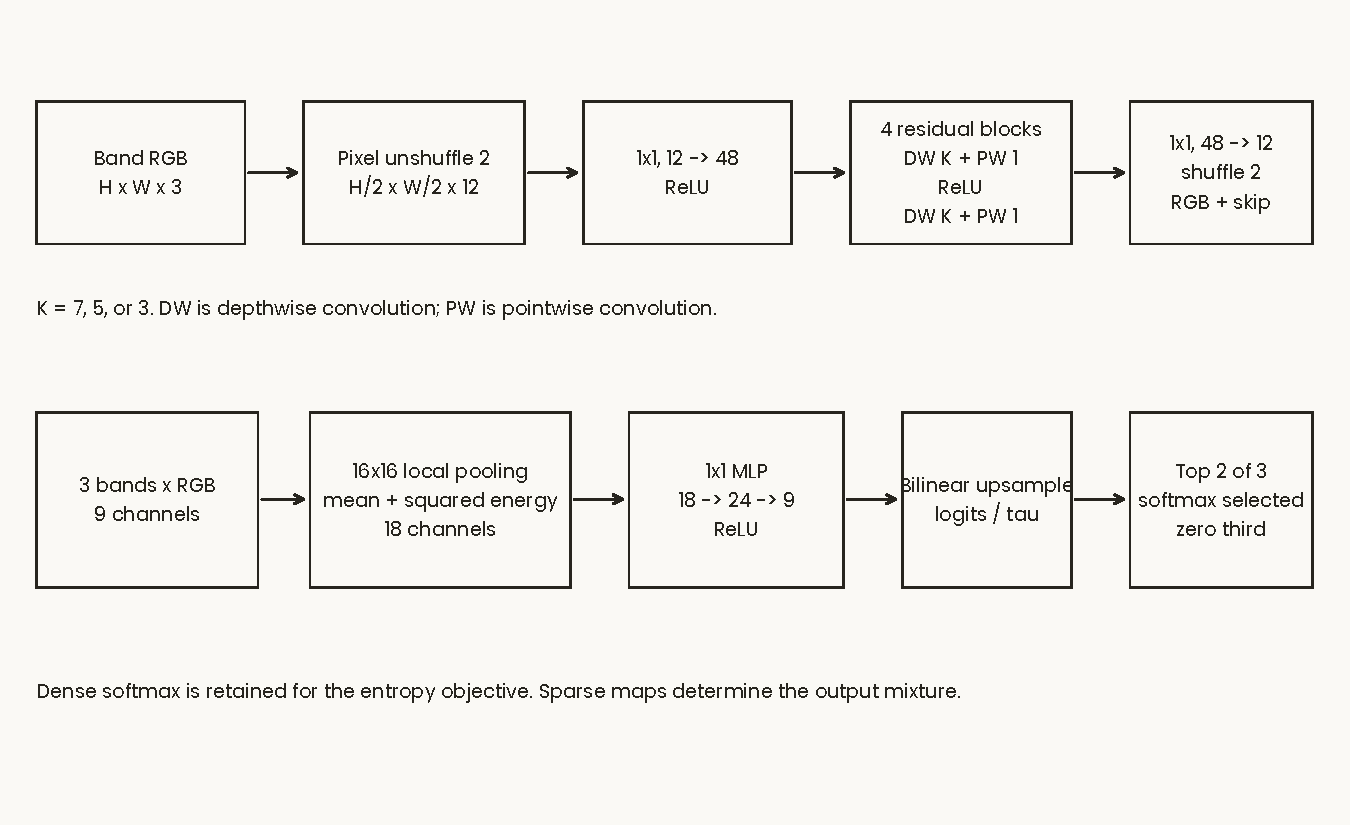
\includegraphics[width=0.9\linewidth]{expert_gate.pdf}
	\caption{Expert and gate operations. Experts use pixel rearrangement and
	depthwise-separable residual blocks; the gate pools band statistics in
	$16\times16$ windows.}
	\label{fig:gate}
\end{figure}

As noted in Section~\ref{sec:lit-moe}, every expert is evaluated before
mixing. Expert outputs at locations with zero weight are computed and then
multiplied by zero. Turning the sparse weights into saved computation would
require tiled conditional dispatch, which we did not implement.

\section{Fusion and Residual Refinement}\label{sec:fusion}

The three weighted band outputs are concatenated into nine channels. A
squeeze-and-excitation block \cite{hu2018se} pools them globally, passes them
through a $9\to3\to9$ bottleneck with a sigmoid, and scales each channel. A
$1\times1$ convolution projects the result to three channels. Three
$3\times3$ convolutions ($3\to16\to16\to3$, ReLU between them) refine it, and
the output is added to the degraded input as in Equation~\eqref{eq:out}.
Predicting a residual rather than the image itself is the central lesson of
DnCNN \cite{zhang2017dncnn}, and it lets the network start from the identity.

\section{Training Objective}\label{sec:loss}

The loss has three terms:
\begin{equation}
	\mathcal{L} = \mathcal{L}_\text{char}
	+ 0.05\,\mathcal{L}_\text{freq}
	+ \lambda_\text{ent}(t)\,\mathcal{L}_\text{ent}.
	\label{eq:loss}
\end{equation}

The Charbonnier loss \cite{charbonnier1994} is a smooth variant of L1,
\begin{equation}
	\mathcal{L}_\text{char} = \operatorname{mean}\sqrt{(\hat f - f)^2 + \varepsilon^2},
	\qquad \varepsilon = 10^{-3},
\end{equation}
which behaves like L2 near zero and like L1 for large errors.

The frequency term is the mean absolute value of the orthonormal FFT of the
prediction error, $\mathcal{L}_\text{freq} = \operatorname{mean}\lvert
\mathcal{F}(\hat f - f)\rvert$. It weights errors at every frequency equally,
which counteracts the tendency of pixel losses to favour the dominant low
frequencies.

The entropy term is the negative dense routing entropy, summed over bands and
averaged over the batch and pixels:
\begin{equation}
	\mathcal{L}_\text{ent} = \sum_b \operatorname{mean}_{n,u,v}\sum_e p_{b,e}\log p_{b,e}.
\end{equation}
Minimising it maximises entropy, which keeps all three experts in use early
in training so that none of them is starved of gradient. A constant entropy
bonus would, however, push the router towards uniform weights forever, which
is the opposite of what we want to observe. The coefficient therefore decays
linearly, $\lambda_\text{ent}(t) = 0.01\,(1 - t/T)$, reaching zero at the
last update $T$. Because the sign of this term is easy to flip by accident,
the verification suite checks that it decreases as the weights approach
uniform. DnCNN and FFDNet are trained with the same Charbonnier and
frequency terms and no entropy term.

\section{Model Size and Complexity}\label{sec:size}

Table~\ref{tab:params} breaks down the 97,088 parameters. Almost all of them
are in the three experts; the gate, fusion and refinement stages together
account for under four thousand.

\begin{table}[htbp]
	\centering
	\caption{\fcsg{} parameter breakdown.}
	\label{tab:params}
	\begin{tabular}{@{}lr@{}}
		\toprule
		Module & Parameters \\
		\midrule
		Shared $7\times7$ expert            & 39,228 \\
		Shared $5\times5$ expert            & 30,012 \\
		Shared $3\times3$ expert            & 23,868 \\
		Spatial gate ($18\to24\to9$)        & 681 \\
		SE fusion and $9\to3$ projection    & 96 \\
		Residual refinement                 & 3,203 \\
		\midrule
		Total                               & 97,088 \\
		\bottomrule
	\end{tabular}
\end{table}

For compute we profile multiply-accumulate operations (MACs) with
\texttt{thop}, count each MAC as two floating-point operations, and add an
estimate of $12 \times 5N\log_2 N$ for the forward and inverse FFTs, with
$N = 256^2$. Small elementwise operations are not counted. Under this
convention a $256\times256$ forward pass costs 4.66 GMACs, or 9.39 GFLOPs
including the FFT estimate, inside the 10 GFLOP limit. The same convention is
applied to the baselines. As Chapter~\ref{ch:results} shows, this count turned
out to be a poor predictor of actual running time.
